\documentclass[10pt,a4paper]{article}
\usepackage[latin1]{inputenc}
\usepackage[english]{babel}
\usepackage{amsmath}
\usepackage{amsfonts}
\usepackage{amssymb}
\usepackage{makeidx}
\usepackage{graphicx}
\usepackage{hyperref}
\usepackage[left=2cm,right=2cm,top=2cm,bottom=2cm]{geometry}

\author{Anders Dall'Osso Teigset}
\title{Puffer mechanism}

\begin{document}
\maketitle
%Summary
\newpage
\section{Summary}
\newpage
\tableofcontents
\newpage
\section{Introduction}
A load break switch should be able to interrupt currents less or equal the maximum load current in a distribution system. When interrupting a current the two contacts which a switch consists of start separating producing a gap between each other. Normally the current is not interrupted by this and an electrical arc ignites and burns in the contact gap \cite{bib:HVEbreak}. The arc consists of plasma, which is a mixture of negative and positive ions as well as electrons. Due to the energy dissipation produced by the arc the temperature in the plasma is very high. The electrical conductivity of the plasma channel is dependent of the temperature produced by the arc. When a high current is flowing it is almost a perfect conductor, but at low temperatures the conductivity is much poorer.

An AC-current have a natural zero crossing, as the current approaches this point the arc will start cooling and extinguish if properly cooled at this point of the power cycle. The working principle of a switchgear is to cool the arc sufficiently when the current approaches zero and then quench the arc when the current is zero. At this moment the current is interrupted and a voltage builds up across the open contacts. This voltage is called the recovery voltage. The steepness and amplitude of the recovery voltage \cite{bib:HVEbreak} and the design of the switchgear will decide if a new arc ignites between the contacts after the current zero. If an arc re-ignites ether by a thermal or a dielectric breakdown the interruption has failed. 

Upon till now SF$_6$ and vacuum based technology have been dominating the compact medium-voltage switchgear market. Air insulated switchgear does exists but they are space consuming and are not applicable for use in a compact substation design. A compact substation is one of the most common designs for substations in the medium-voltage level of the distribution system. Figure \ref{fig:compact substation} displays a compact substation which can be used in the medium-voltage distribution system. The switchgear is a module that can be detached from the compact substation and removed trough its front panel. As figure \ref{fig:compact substation} shows there are a limited amount of space available for the switchgear. Therefore the main challenge for an air insulated switchgear design for this kind of application is set by the amount of space available in the compact substation.

\begin{figure} [h]
\centering
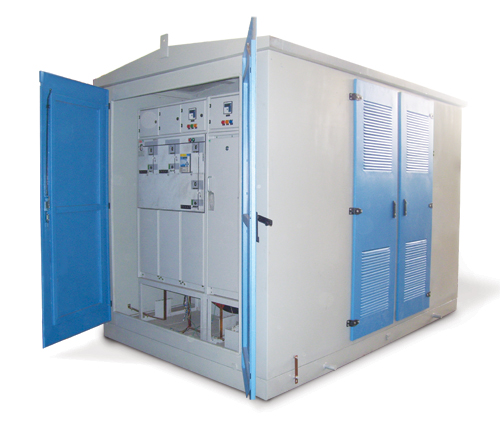
\includegraphics[scale=0.5]{Bilder/Introduction/general_substation.jpg}
\caption{Compact substation with open front panel \cite{bib:comSub}} \label{fig:compact substation}
\end{figure}

The main choice of interrupting media in switchgear has been SF$_6$ since its discovery in the 1970ies. The gas exhibits many properties which is well suited for an isolation gas. It is highly electron negative which gives it good dielectric strength and arc-interrupting capabilities. The breakdown voltage of SF$_6$ is almost three times higher than air at atmospheric pressure \cite{bib:SF6PI}. It has excellent heat transfer properties as an interrupting medium \cite{bib:SF6PI}. The gas also reforms itself when dissociated under the high temperature conditions in an electrical arc. SF$_6$ produces no polymerization, carbon or other conductive deposits during arcing. It is also chemically compatible with most insulation materials and conductive materials \cite{bib:SF6PI}. The gas is also well suited for use in low temperature environments since its boiling point is fairly low even at high pressures. The gas in its stable form is nontoxic, non-flammable and non-explosive. It is also thermally stable and do not decompose at normal operating temperatures for a closed switch \cite{bib:SF6PI}. SF$_6$ based switchgear tends to be cheap to produce relative to other designs, and the gas itself is also affordable at today prices.


SF$_6$ have some disadvantages, when exposed to electrical discharge or arcing it forms highly toxic and corrosive compounds \cite{bib:SF6PI}. It is also hard to remove non-polar contaminants like air and its breakdown voltage is sensitive to water vapour and conductive particles. However it biggest downside is probably that it is an effective infrared absorber. This makes it a strong greenhouse gas \cite{bib:SF6PI} and it is regarded to be almost $20000$ times as potent as CO$_2$.

0.4 \% of the greenhouse gas emissions in Norway is due to SF$_6$ and is mainly used in switchgear or other high voltage equipment \cite{bib:KlimaKur2020}. In Norway the use of SF$_6$ is regulated through a voluntary contract between the environmental department and the end user, mainly the power companies \cite{bib:KlimaKur2020}. If a compatible air based switchgear design is released on the market it can be assumed that the power companies will be interested in the new technology. It is also possible that the government will restrict the use of SF$_6$ gas if the private sector do not follow the guidelines of the environmental department.

A test switch have been developed which allows adjustment of many design parameter such as nozzle and contact geometry, contact movement and gas pressure. The contacts consist of one female contact, or tulip and one male contact, or pin. The tulip is immovable, while the pin can be opened by a spring trigged by an electromagnet. Previous results have shown that most of the successful interruptions have occurred when the pin is outside the nozzle \cite{bib:CIAMVLBS}. Cold air simulations done by Nina Sasaki Aanensen of the different geometries have shown that volumetric flow of air is much lower when the pin is inside the nozzle. The results from previous testing and cold air simulations might suggest that the pin is clogging the nozzle and preventing a good air flow. Therefore a new nozzle geometry has been designed with a doughnut area, the area between the nozzle and the pin, which is bigger than the area of the pin. This is assumed to give a volumetric flow of air that is almost the same when the pin is inside the nozzle as well as outside. The theory has been verified by cold air simulations. However the clogging effect generated by an arc has not been taken into account and it is expected that this will have an impact on the volumetric flow. Two nozzles have been constructed of the new nozzle geometry one with an doughnut area of $44 \ mm^2$ and the other one with an area of $66 \ mm^2$. It is expected that the speed of the air will be constant and the volumetric flow will increase with the doughnut area. This will give an opportunity to test which of these parameters that influence the current interruption capabilities the most.

Several different nozzle geometries are going to be tested and it is assumed that the chance for a successful current interruption inside the nozzle will be approximately the same as outside the nozzle. Since the size of the arc compared to the pin will vary between the different nozzle geometries and current amplitudes, a clogging effect is assumed to occur and might be revealed as an lower interruption success rate for certain geometries.

\newpage
\section{Theory}
\subsection{Switchgear design}
\subsubsection{General design}
Switchgear can be divided into four main categories:
\begin{itemize}
\item Disconnector switch
\item Load Break Switch
\item Circuit Switch
\item Earthing Switch
\end{itemize}
This report will focus on the load break switch (LBS) design. A LBS is a switchgear design to be able to interrupt currents with magnitude that is equal or less than the rated maximum continuous current in the power system. A LBS must fulfil the following demands to meet the requirements of the area of application:

\begin{itemize}
\item When closed:
	\begin{itemize}
		\item It must act as an perfect conductor.
		\item Be capable to interrupt any currents that may arise, without generating too high over-voltages. 
	\end{itemize}
\item When open:
	\begin{itemize}
		\item It must be an perfect isolator.
		\item be able to close without welding the contacts together, event under short-circuit conditions.
	\end{itemize}
\end{itemize}


A switchgear will need to contain two sets of contacts to meet the requirements above. This is done by having one set of main contacts and one set of arcing contacts. These sets have different behaviour and roles when breaking a current and are connected in parallel. In a LBS the main contacts primary function is to assure that the switch in closed position acts as a perfect conductor with as little as possible contact resistance. Copper  or aluminium is often as material in the main contact. Sometimes the contact surface is plated with tin, gold, silver or platinum to ensure a low contact resistance between the main contacts. This contact is the first contact to open and the last one to close. This is to ensure that an arc do not start to burn between the contact. This is of great importance because the materials a main contact is made out of is usually not very heat resistant and might get damaged by the arc.

The other set of contact is the arcing contact. The arcing contact is the last contact to open, and the first one to close. Therefore this contact will need to withstand the harsh conditions that happens when an arc burns between them. The contact points need to withstand high temperatures, arc erosion, welding and other stresses that may apply when closing or opening an energized contact. Aluminium and copper is not fit for this tasks since they will melt or erode from stresses of an arc. It is common to use composites of metals with good electrical conduction with heat resistant oxides. The problem with this kinds of composites is that the have a considerable resistance. Without the main contact in parallel with the arcing contact, the losses and the heat generation in the switchgear would be to large and might damage the arcing contact over time.

\subsubsection{Test switch}
A new medium voltage laboratory for load break switch development have been designed with the possibilities to vary important design parameters for a load break switch. When the industry develops switchgear technology they tend to alter several different parameters at the same time. For instance, if they wish to alter the speed of the airflow in a puffer LBS, they might increases the separation speed of the contacts, since these functions often are linked in a puffer design. This will also result in a higher pressure not only and not only a higher volumetric flow. This will make it hard to conclude which parameter that was the most critical for a successful interruption. Therefore a laboratory switch have been design where each of the different parameters can be adjusted without changing other critical parameter. This will make systematic researching possible and optimisation of certain designs criteria, like dimensions, will be a lot simpler.

\begin{figure} [h]
\centering
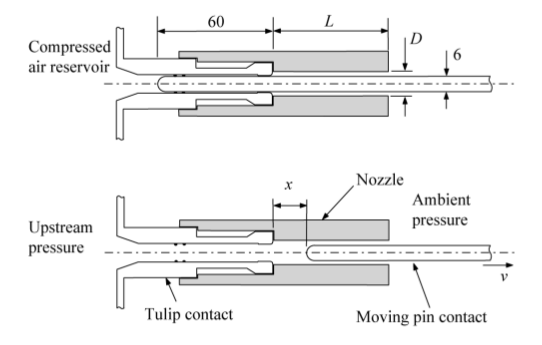
\includegraphics[scale=0.5]{Bilder/Theory/SchematicTestSwitch.png}
\caption{Test switch} \label{fig:testSwitch}
\end{figure}

Figure \ref{fig:testSwitch} shows the physical appearance of the switch and how the different parameter can be adjusted. BLA BLA TAKE A PICTURE OF THE SWITCH, WRITE SOME NUMBERS ON IT. TAKE ABOUT THEM AND WITCH PARAMETERS THAT CAN BE ADJUSTED.

\begin{figure} [h]
\centering
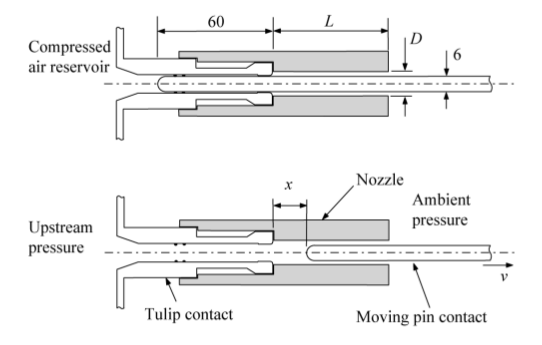
\includegraphics[scale=0.5]{Bilder/Theory/SchematicTestSwitch.png}
\caption{Tulip, nozzle and pin, L and D is the length and inner diameter of the nozzle, x is contact position. Dimensions are in millimetres.   \cite{bib:CIAMVLBS}} \label{fig:SchematicTestSwitch}
\end{figure}

Figure \ref{fig:SchematicTestSwitch} display the former nozzle geometries and it can be clearly seen from this picture that the doughnut area is smaller than the tulip area. It is possible that this will give a clogging effect when the pin is inside the nozzle and result in a poorer airflow and interrupting capabilities for this situation. In figure \ref{fig:differentGeometries} the different contact geometries that have been made is shown. Geometries a1, b1, and c1 have been tested and the results showed that most of the successful interruptions happen when the pin was outside the nozzle. It is possible that this is the result of a clogging effect that takes place between the nozzle and pin. Therefore geometries b2 and c2 was created. The geometries is similar to b1 and c1 since they have the same nozzle area, respectively $44 \ mm^2$ and $66 \ mm^2$. The volumetric airflow will however be smaller for b2 and c2 because it have been created a choking point in the tulip. 

\begin{figure} [h]
\centering
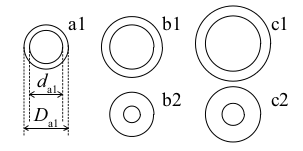
\includegraphics[scale=0.6]{Bilder/Theory/differentGeometries.png}
\caption{Different contact geometries \cite{bib:CIAMVLBS}} \label{fig:differentGeometries}
\end{figure}

It is expected that b2 and c2 will need a higher pressure than b1 and c1 to perform a successful interruption, due to the lower airflow. However it is expected that they will have an equal successrate no matter if the pin is inside the nozzle or outside the nozzle.
\newpage
\subsection{Interrupting currents}
\subsubsection{Switching scenarios}
\subsubsection{Ionisation processes}
\subsubsection{Temperature profile for an electrical arc}
\subsubsection{The difference between air and SF$_6$ as interrupting medium}
\newpage
\subsection{Environmental impacts of SF$_6$ from electrical power industries}
SF$_6$ is an effective infrared absorber and have a long lifetime in the atmosphere. This makes it a strong greenhouse gas. Because of the increase in commercial use since the 1970s the production of the gas have steadily increased. This have resulted in a rise of the SF$_6$ concentration in the atmosphere from barely measurable quantities in the 1980s \cite{bib:SF6PI} to sett inn nytt tall her!
\newpage

\begin{thebibliography}{10}


\bibitem{bib:HVEbreak} \textit{M. Runde}, \textit{Current Interruption in Power Grids}. Trondheim: Norwegian University of Science and Technology, 2013, p. 1-2 - 1-6

\bibitem{bib:SF6PI} \textit{L.G. Christophorou, J. K. Olthoff, and R.J. Van Brunt}, "\textit{Sulfur Hexafluoride and the Electric Power Industry}", \textit{IEEE Electrical Insulation Magazine, vol. 13, No. 5, pp. 20-24}, Oct. 1997.

\bibitem{bib:comSub} \textit{amesimpex.com}, \url{http://www.amesimpex.com/images/unitised_sub_002.jpg}, \textit{26.9.2013}

\bibitem{bib:CIAMVLBS} \textit{E. Jonsson, N. S. Aanensen and M. Runde}, "\textit{Current Interruption in Air for a Medium Voltage Load Break Switch}", \textit{IEEE Trans. Power Delivery}, to be published.

\bibitem{bib:KlimaKur2020} "\textit{KLIMAKUR2020}", Oslo: Klima- og forurensningsdirektoratet, 2010, p. 197
\end{thebibliography}
\end{document}